\uuid{nSSt}
\chapitre{Fonction de plusieurs variables}
\sousChapitre{Extremums locaux}
\titre{Problème concret}
\theme{optimisation}
\auteur{Jean-François Culus}
\datecreate{2024-10-21}
\organisation{AMSCC}
\contenu{

\texte{On désire fabriquer par une imprimante 3D une boite ayant la forme d'un parallélépipède rectangle, sans couvercle sur le dessus. Le volume de cette boite doit être égal à $0,5m^3$.}


\question{ Pour minimiser la quantité de matière utilisée, on désire que la somme des aires des faces soit minimale. Quelles dimensions doit-on choisir pour fabriquer la boite ? }
\smallskip
\texte{ \\ {\bf Indication:} Se ramener à un problème d'optimisation d'une fonction de deux variables.  }

\reponse{Notons $x,y$ et $z$ les dimensions de la boite. 
Son volume (la contrainte) est donc égale à $xyz=0,5$. 
On souhaite minimiser la fonction $f(x,y,z)=xy+2xz+2yz$. 
Comme $z=\frac{1}{2xy}$, nous savons que ce problème revient à rechercher le minimum de la fonction $g(x,y)=xy+\frac{1}{x}+\frac{1}{y}$ sur l'ouvert $U=\mathbb{R}_+^* \times \mathbb{R}_+^*$. 
Les dérivées partielles sont alors:
$$ \frac{\partial g}{\partial x}(x,y)=y-\frac{1}{x^2} ~~\text{ et }~~
\frac{\partial g}{\partial y}(x,y)=x - \frac{1}{y^2}$$
L'unique point critique sur $U$ est alors le point $(1,1)$. 
\\ Pour vérifier que c'est bien un minimum, on peut éventuellement calculer la hessienne. 
$$H_g(x,y)= \begin{vmatrix} 
2x^{-3} & 1 \\ 1 & 2y^{-3} 
\end{vmatrix} $$
Ainsi, $det(H_f(1,1))=3>0$: ainsi, $f$ atteint bien un extremum en $(1,1)$ et comme 
$\frac{\partial^2 g}{\partial x^2}(1,1)>0$, $g$ atteint un minimum en $(1,1)$. 
Ainsi, la boite a une aire minimale pour les valeurs $x=1$, $y=1$ et $z=\frac{1}{2}$.

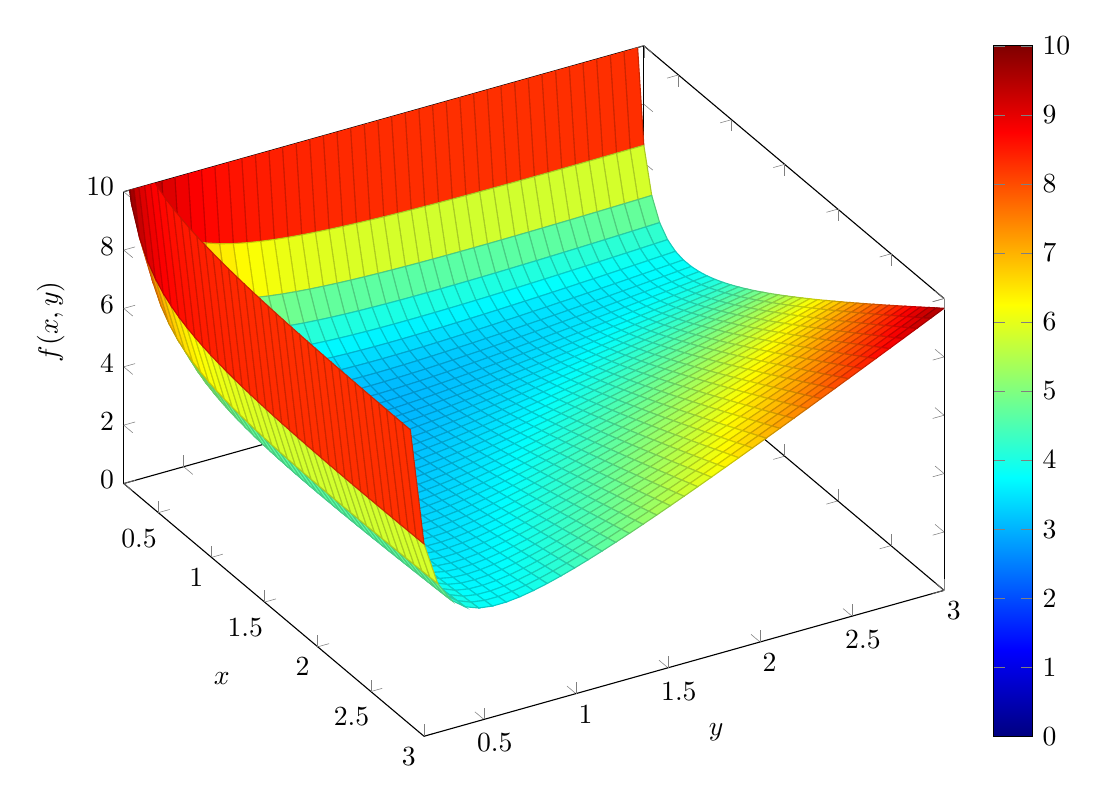
\begin{tikzpicture}
    \begin{axis}[
        width=12cm, % largeur du graphique
        view={60}{45}, % angle de vue
        domain=0.1:3, y domain=0.1:3, % limites pour x et y (éviter 0)
        samples=40, % nombre de points pour tracer le graphique
        xlabel=$x$, ylabel=$y$, zlabel={$f(x, y)$},
        colormap/jet, % colormap avec plus de couleurs vives
        %shader=interp, % shading interpolé
        colorbar, % afficher une barre de couleur
        zmin=0, % limite inférieure de z
        zmax=10, % limite supérieure de z
        point meta min=0, point meta max=10, % ajuster l'étendue de la colormap
    ]
        \addplot3[
            surf,
        ]
        {x*y + 1/x + 1/y};
    \end{axis}
\end{tikzpicture}

}

}